
\documentclass[12pt,a4paper, oneside]{extreport}

%%%%%%%%%% Математика %%%%%%%%%%
\usepackage{amsmath,amsfonts,amssymb,amsthm,mathtools}
% Показывать номера только у тех формул, на которые есть \eqref{} в тексте.
%\mathtoolsset{showonlyrefs=true}
%\usepackage{leqno} % Нумерация формул слева
%\usepackage{tipa} %Для формулки из логитов


\usepackage{hyphenat}

%%%%%%%%%% Шрифты %%%%%%%%
\usepackage[english, russian]{babel} % выбор языка для документа
\usepackage[utf8]{inputenc} % задание utf8 кодировки исходного tex файла
\usepackage[X2,T2A]{fontenc}        % кодировка
%
\usepackage{fontspec}         % пакет для подгрузки шрифтов
\setmainfont{Times New Roman}       % задаёт основной шрифт документа

\usepackage{unicode-math}      % пакет для установки математического шрифта
%\setmathfont{Asana-Math.otf}    % шрифт для математики

% Конкретный символ из конкретного шрифта
% \setmathfont[range=\int]{Neo Euler}


%%%%%%%%%% Работа с картинками %%%%%%%%%
\usepackage{graphicx}                  % Для вставки рисунков
\usepackage{graphics}
\graphicspath{{images/}{pictures/}}    % можно указать папки с картинками
\usepackage{wrapfig}                   % Обтекание рисунков и таблиц текстом


%%%%%%%%%% Работа с таблицами %%%%%%%%%%
\usepackage{tabularx}            % новые типы колонок
\usepackage{tabulary}            % и ещё новые типы колонок
\usepackage{array,delarray}      % Дополнительная работа с таблицами
\usepackage{longtable}           % Длинные таблицы
\usepackage{multirow}            % Слияние строк в таблице
\usepackage{float}               % возможность позиционировать объекты в нужном месте

\usepackage{booktabs}            % таблицы как в книгах

% Заповеди из документации к booktabs:
% 1. Будь проще! Глазам должно быть комфортно
% 2. Не используйте вертикальные линни
% 3. Не используйте двойные линии. Как правило, достаточно трёх горизонтальных линий
% 4. Единицы измерения - в шапку таблицы
% 5. Не сокращайте .1 вместо 0.1
% 6. Повторяющееся значение повторяйте, а не говорите "то же"
% 7. Есть сомнения? Выравнивай по левому краю!

%  вычисляемые колонки по tabularx
\newcolumntype{C}{>{\centering\arraybackslash}X}
\newcolumntype{L}{>{\raggedright\arraybackslash}X}
\newcolumntype{Y}{>{\arraybackslash}X}
\newcolumntype{Z}{>{\centering\arraybackslash}X}


%%%%%%%%%% Графика и рисование %%%%%%%%%%
\usepackage{tikz, pgfplots}      % язык для рисования графики из latex'a

%%%%%%%%%% Гиперссылки %%%%%%%%%%
\usepackage{xcolor}              % разные цвета

\usepackage{hyperref}
\hypersetup{
	unicode=true,           % позволяет использовать юникодные символы
	colorlinks=true,       	% true - цветные ссылки, false - ссылки в рамках
	urlcolor =blue,         % цвет ссылки на url
	linkcolor=black,        % внутренние ссылки
	citecolor=black,        % на библиографию
	breaklinks              % если ссылка не умещается в одну строку, разбивать ли ее на две части?
}


%%%%%%%%%% Другие приятные пакеты %%%%%%%%%
\usepackage{multicol}       % несколько колонок
\usepackage{verbatim}       % для многострочных комментариев
\usepackage{cmap} % для кодировки шрифтов в pdf

\usepackage{enumitem} % дополнительные плюшки для списков
%  например \begin{enumerate}[resume] позволяет продолжить нумерацию в новом списке

\usepackage{todonotes} % для вставки в документ заметок о том, что  осталось сделать
% \todo{Здесь надо коэффициенты исправить}
% \missingfigure{Здесь будет Последний день Помпеи}
% \listoftodos --- печатает все поставленные \todo'шки



%%%%%%%%%%%%%% ГОСТОВСКИЕ ПРИБАМБАСЫ %%%%%%%%%%%%%%%

%%% размер листа бумаги
\usepackage[paper=a4paper,top=15mm, bottom=15mm,left=35mm,right=10mm,includehead]{geometry}


\usepackage{setspace}
\setstretch{1.5}     % Межстрочный интервал
\setlength{\parindent}{1.25cm} % Красная строка.


%\flushbottom       % Эта команда заставляет LaTeX чуть растягивать строки, чтобы получить идеально прямоугольную страницу
\righthyphenmin=2  % Разрешение переноса двух и более символов
\widowpenalty=10000  % Наказание за вдовствующую строку (одна строка абзаца на этой странице, остальное --- на следующей)
\clubpenalty=10000  % Наказание за сиротствующую строку (омерзительно висящая одинокая строка в начале страницы)
\tolerance=1000     % Ещё какое-то наказание.


% Нумерация страниц сверху по центру
\usepackage{fancyhdr}
\pagestyle{fancy}
%\fancyhead{ } % clear all fields
%\fancyfoot{ } % clear all fields
\fancyhf{}
\fancyhead[R]{Касьянова Ксения (СМАР19)}
\fancyfoot[C]{\thepage}
% Чтобы не прорисовывалась черта!
\renewcommand{\headrulewidth}{0pt}


% Нумерация страниц с надписью "Глава"
\usepackage{etoolbox}
\patchcmd{\chapter}{\thispagestyle{plain}}{\thispagestyle{fancy}}{}{}


%%% Заголовки
\usepackage[indentfirst]{titlesec}{\raggedleft}
% Заголовки по левому краю
% опция identfirst устанавливает отступ в первом абзаце



% В Linux этот пакет сделан косячно. Исправляет это следующий непонятный кусок кода.
\makeatletter
\patchcmd{\ttlh@hang}{\parindent\z@}{\parindent\z@\leavevmode}{}{}
\patchcmd{\ttlh@hang}{\noindent}{}{}{}
\makeatother


% Редактирования Глав и названий
\titleformat{\chapter}
{\normalfont\large\bfseries}
{\thechapter }{0.5 em}{}

% Редактирование ненумеруемых глав chapter* (Введение и тп)
\titleformat{name=\chapter,numberless}
{\centering\normalfont\bfseries\large}{}{0.25em}{\normalfont}

% Убирает чеканутые отступы вверху страницы
\titlespacing{\chapter}{0pt}{-\baselineskip}{\baselineskip}

% Более низкие уровни
\titleformat{\section}{\bfseries}{\thesection}{0.5 em}{}
\titleformat{\subsection}{\bfseries}{\thesubsection}{0.5 em}{}

\titlespacing*{\section}{0 pt}{\baselineskip}{\baselineskip}
\titlespacing*{\subsection}{0 pt}{\baselineskip}{\baselineskip}


% Содержание. Команды ниже изменяют отступы и рисуют точечки!
\usepackage{titletoc}

\titlecontents{chapter}
[1em] %
{\normalsize}
{\contentslabel{1 em}}
{\hspace{-1 em}}
{\normalsize\titlerule*[10pt]{.}\contentspage}

\titlecontents{section}
[3 em] %
{\normalsize}
{\contentslabel{1.75 em}}
{\hspace{-1.75 em}}
{\normalsize\titlerule*[10pt]{.}\contentspage}

\titlecontents{subsection}
[6 em] %
{\normalsize}
{\contentslabel{3 em}}
{\hspace{-3 em}}
{\normalsize\titlerule*[10pt]{.}\contentspage}


% Правильные подписи под таблицей и рисунком
% Документация к пакету на русском языке!
\usepackage[tableposition=top, singlelinecheck=false]{caption}
\usepackage{subcaption}


\DeclareCaptionStyle{base}%
[justification=centering,indention=0pt]{}
\DeclareCaptionLabelFormat{gostfigure}{Рисунок #2}
\DeclareCaptionLabelFormat{gosttable}{Таблица #2}

\DeclareCaptionLabelSeparator{gost}{~---~}
\captionsetup{labelsep=gost}

\DeclareCaptionStyle{fig01}%
[margin=5mm,justification=centering]%
{margin={3em,3em}}
\captionsetup*[figure]{style=fig01,labelsep=gost,labelformat=gostfigure,format=hang}

\DeclareCaptionStyle{tab01}%
[margin=5mm,justification=centering]%
{margin={3em,3em}}
\captionsetup*[table]{style=tab01,labelsep=gost,labelformat=gosttable,format=hang}


% межстрочный отступ в таблице
\renewcommand{\arraystretch}{1.2}



% многостраничные таблицы под РОССИЙСКИЙ СТАНДАРТ
% ВНИМАНИЕ! Обязательно за CAPTION !
\usepackage{fr-longtable}



%Более гибкие спсики
\usepackage{enumitem}
% сообщаем окружению о том, что существует такая штук как нумерация русскими буквами.
\makeatletter
\AddEnumerateCounter{\asbuk}{\russian@alph}{щ}
\makeatother


%%% ГОСТОВСКИЕ СПИСКИ

% Первый тип списков. Большая буква.
\newlist{Enumerate}{enumerate}{1}

\setlist[Enumerate,1]{labelsep=0.5em,leftmargin=1.25em,labelwidth=1.25em,
	parsep=0em,itemsep=0em,topsep=0ex, before={\parskip=-1em},label=\arabic{Enumeratei}.}


% Второй тип списков. Маленькая буква.
\setlist[enumerate]{label=\arabic{enumi}),parsep=0em,itemsep=0em,topsep=0.75ex, before={\parskip=-1em}}


% Третий тип списков. Два уровня.
\newlist{twoenumerate}{enumerate}{2}
\setlist[twoenumerate,1]{itemsep=0mm,parsep=0em,topsep=0.75ex,, before={\parskip=-1em},label=\asbuk{twoenumeratei})}
\setlist[twoenumerate,2]{leftmargin=1.3em,itemsep=0mm,parsep=0em,topsep=0ex, before={\parskip=-1em},label=\arabic{twoenumerateii})}


% Четвёртый тип списков. Список с тире.
\setlist[itemize]{label=--,parsep=0em,itemsep=0em,topsep=0ex, before={\parskip=-1em},after={\parskip=-1em}}


%%% WARNING WARNING WARNIN!
%%% Если в списке предложения, то должна по госту стоять точка после цифры => команда Enumerate! Если идет перечень маленьких фактов, не обособляемых предложений то после цифры идет скобка ")" => команда enumerate! Если перечень при этом ещё и двууровневый, то twoenumerate.




%%%%%%%%%% Список литературы %%%%%%%%%%

%\usepackage[%
%backend=biber, %подключение пакета biber (тоже нужен)
%bibstyle=gost-numeric, %подключение одного из четырех главных стилей biblatex-gost
%sorting=ntvy, %тип сортировки в библиографии
%]{biblatex}

\usepackage[backend=biber,style=gost-numeric, maxbibnames=9,maxcitenames=2,uniquelist=false, babel=other]{biblatex}



% Справка по 4 главным стилям для ленивых:
% gost-inline  ссылки внутри теста в круглых скобках
% gost-footnote подстрочные ссылки
% gost-numeric затекстовые ссылки
% gost-authoryear тоже затекстовые ссылки, но немного другие

% Подробнее смотри страницу 4 документации. Она на русском.

% Ещё немного настроек
\DeclareFieldFormat{postnote}{#1} %убирает с. и p.
\renewcommand*{\mkgostheading}[1]{#1} % только лишь убираем курсив с авторов






\begin{document} % Начала документа



\chapter{ДЗ-02}


\section{Задача 1.}


\subsection{Logit-модель.}

Создадим бинарную переменную \texttt{crime86}: 0 - если не был арестован,  1 - если был арестован хоть раз. 

\begin{verbatim}
generate crime86: crime86 = narr86>0
\end{verbatim}

Построим логит для \texttt{crime86}: 

\begin{verbatim}
logit crime86 pcnv avgsen tottime ptime86 qemp86 inc86 durat black hispan born60
\end{verbatim}

\begin{figure}[htb]
	\centering
	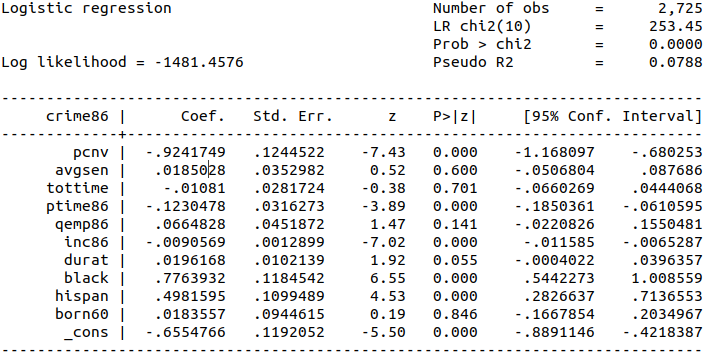
\includegraphics[width=1\linewidth]{screenshot001}
%	\caption{}
	\label{fig:screenshot001}
\end{figure}

Получим оценку \texttt{nocrime} для каждого наблюдения того, что индивидуум не будет ни разу арестован: 

\begin{verbatim}
predict prediction
generate nocrime: nocrime = 1-prediction
\end{verbatim}


\subsection{График долей ошибок I-II рода.}

Посчитаем доли ошибок I рода (\texttt{fpr}) и II рода (\texttt{fnr}) и построим график 
 
\begin{verbatim}
rocreg crime86 prediction, noboot
generate fpr: fpr = \_fpr\_prediction
generate fnr: fnr = 1-_roc_prediction
twoway (scatter fpr fnr), xsize(5) ysize(5)
\end{verbatim}

\begin{figure}[htb]
	\centering
	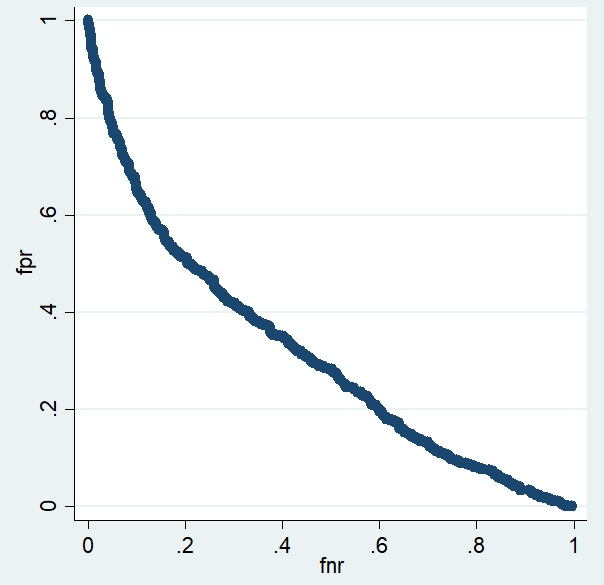
\includegraphics[width=0.7\linewidth]{screen}
	%	\caption{}
	\label{fig:screenshot001}
\end{figure}



\subsection{Poisson count model.}


Построим модель Пуассона для \texttt{narr86}: 

\begin{verbatim}
poisson narr86 pcnv avgsen tottime ptime86 qemp86 inc86 durat black hispan born60
\end{verbatim}

\begin{figure}
	\centering
	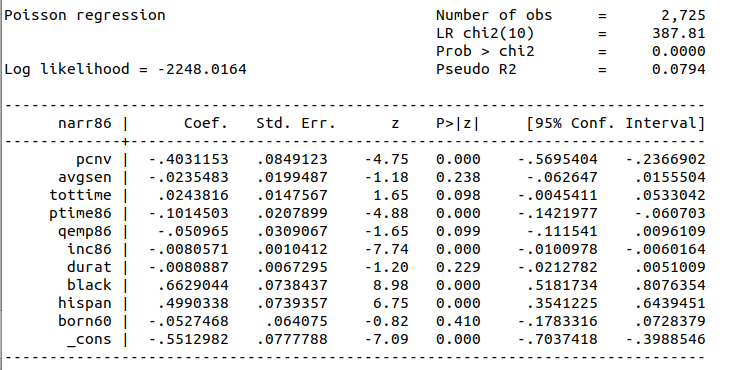
\includegraphics[width=1\linewidth]{screenshot002}
%	\caption{}
	\label{fig:screenshot002}
\end{figure}

Посчитаем, сколько раз эта модель верно определяет, был ли арестован человек:

\begin{verbatim}
predict prediction_pois, n

count if prediction_pois>0.6 & narr86>=1
244

count if prediction_pois<= 0.6 & narr86==0
1,723
\end{verbatim}

Сравним с логит-моделью:

\begin{verbatim}
count if prediction>0.4 & crime86==1
226

count if prediction<=0.4 & crime86==0
1,711
\end{verbatim}

Модель Пуассона позволяет получить более  точные прогнозы, как для арестованных, так и нет.

В обеих моделях значимые (на 1\% уровне значимости) переменные влияют на вероятность ареста с одинаковым знаком.

Зачастую модель регрессии Пуассона плохо соответствует счетным данным,  поскольку распределение Пуассона задается единственным параметром $(\mu)$. 
Другим недостатком является то, что модель Пуассона подразумевает равенство дисперсии и математического ожидания, в то время как в счетных данных дисперсия обычно превышает среднее.

Одно из последствий такого однопараметрического моделирования заключается в том, что вероятность нулевых значений, предсказанная по модели Пуассона, значительно ниже, чем их доля в выборке, что называется проблемой избыточных нулевых значений.


Во избежание проблем  избыточных нулевых значений и завышенной дисперсии лучше использовать модель бинарного выбора.

\section{Задача 2.}


\subsection{}

$x'\hat{\beta_2} = -0.35474*90 - 0.1655*9+ 0.2655*15.52+0-0.46766*2.9957+1.5136  = -0.44697 $

$P(at16=2) \dfrac{\exp{-0.44697}}{1+0.639564+0.33202} = 0.324391$

$x'\hat{\beta_3} = -0.0451-0.29184*9+0.2189*15.52-0.78503*2.9435= -1.10256 $

$P(at16=3) \dfrac{\exp{-1.10256}}{1+0.639564+0.33202} = 0.168403$

$P(at16=1) = 1 - P(at16=2) - P(at16=3)  =  0.5072064 $


\subsection{}

$ P(at16|girl) = \dfrac{0.653572}{1+0.653572+0.396036} = 0.318877$

$x'\hat{\beta_3}  = -0.4253 $

$\exp{(x'\hat{\beta_3})}  = 0.653572 $


$x'\hat{\beta_3}  = -0.92625 $

$\exp{{x'\hat{\beta_3}}}  = 0.396036 $

$diff = 0.318877-0.168403=0.150474$


$\ln\dfrac{P(at16=3|girl)}{P(at16=3|boy)} = 0.638447$

\subsection{}


$\dfrac{\partial P(at16=1)}{\partial loginc} = \left[\dfrac{1}{1+ \exp{(x'\beta_2)} + \exp{(x'\beta_3)}} \right]' = $

$ = \dfrac{-1*(-0.639551*0.4676+0.33202*0.78503)}{(1+0.639551+0.33202)^2} = 0.144001$

\subsection{}

Независимость от несущественных альтернатив   (Independence of irrelevant alternatives) -- одна из предпосылок мультиномиальной логистической  модели,  утверждающая, относительная вероятность выбора между одним из двух вариантов не зависит ни от каких дополнительных альтернатив в наборе, другими словами  добавление   еще одного  элемента  к набору вариантов выбора, уменьшит вероятность всех элементов на равную долю.

\end{document}
